%%%%%%%%%%%%%%%%%%%%%%%%%%%%%%%%%%%%%%%%%
% Wenneker Assignment
% LaTeX Template
% Version 2.0 (12/1/2019)
%
% This template originates from:
% http://www.LaTeXTemplates.com
%
% Authors:
% Vel (vel@LaTeXTemplates.com)
% Frits Wenneker
%
% License:
% CC BY-NC-SA 3.0 (http://creativecommons.org/licenses/by-nc-sa/3.0/)
% 
%%%%%%%%%%%%%%%%%%%%%%%%%%%%%%%%%%%%%%%%%

%----------------------------------------------------------------------------------------
%	PACKAGES AND OTHER DOCUMENT CONFIGURATIONS
%----------------------------------------------------------------------------------------

\documentclass[11pt]{scrartcl} % Font size

%%%%%%%%%%%%%%%%%%%%%%%%%%%%%%%%%%%%%%%%%
% Wenneker Assignment
% Structure Specification File
% Version 2.0 (12/1/2019)
%
% This template originates from:
% http://www.LaTeXTemplates.com
%
% Authors:
% Vel (vel@LaTeXTemplates.com)
% Frits Wenneker
%
% License:
% CC BY-NC-SA 3.0 (http://creativecommons.org/licenses/by-nc-sa/3.0/)
% 
%%%%%%%%%%%%%%%%%%%%%%%%%%%%%%%%%%%%%%%%%

%----------------------------------------------------------------------------------------
%	PACKAGES AND OTHER DOCUMENT CONFIGURATIONS
%----------------------------------------------------------------------------------------

\usepackage{amsmath, amsfonts, amsthm} % Math packages

\usepackage{listings} % Code listings, with syntax highlighting

\usepackage[english]{babel} % English language hyphenation

\usepackage{graphicx} % Required for inserting images
\graphicspath{{Figures/}{./}} % Specifies where to look for included images (trailing slash required)

\usepackage{booktabs} % Required for better horizontal rules in tables

\numberwithin{equation}{section} % Number equations within sections (i.e. 1.1, 1.2, 2.1, 2.2 instead of 1, 2, 3, 4)
\numberwithin{figure}{section} % Number figures within sections (i.e. 1.1, 1.2, 2.1, 2.2 instead of 1, 2, 3, 4)
\numberwithin{table}{section} % Number tables within sections (i.e. 1.1, 1.2, 2.1, 2.2 instead of 1, 2, 3, 4)

\setlength\parindent{0pt} % Removes all indentation from paragraphs

\usepackage{enumitem} % Required for list customisation
\setlist{noitemsep} % No spacing between list items

%----------------------------------------------------------------------------------------
%	DOCUMENT MARGINS
%----------------------------------------------------------------------------------------

\usepackage{geometry} % Required for adjusting page dimensions and margins

\geometry{
	paper=a4paper, % Paper size, change to letterpaper for US letter size
	top=2.5cm, % Top margin
	bottom=3cm, % Bottom margin
	left=3cm, % Left margin
	right=3cm, % Right margin
	headheight=0.75cm, % Header height
	footskip=1.5cm, % Space from the bottom margin to the baseline of the footer
	headsep=0.75cm, % Space from the top margin to the baseline of the header
	%showframe, % Uncomment to show how the type block is set on the page
}

%----------------------------------------------------------------------------------------
%	FONTS
%----------------------------------------------------------------------------------------

\usepackage[utf8]{inputenc} % Required for inputting international characters
\usepackage[T1]{fontenc} % Use 8-bit encoding

\usepackage{fourier} % Use the Adobe Utopia font for the document

%----------------------------------------------------------------------------------------
%	SECTION TITLES
%----------------------------------------------------------------------------------------

\usepackage{sectsty} % Allows customising section commands

\sectionfont{\vspace{6pt}\centering\normalfont\scshape} % \section{} styling
\subsectionfont{\normalfont\bfseries} % \subsection{} styling
\subsubsectionfont{\normalfont\itshape} % \subsubsection{} styling
\paragraphfont{\normalfont\scshape} % \paragraph{} styling

%----------------------------------------------------------------------------------------
%	HEADERS AND FOOTERS
%----------------------------------------------------------------------------------------

\usepackage{scrlayer-scrpage} % Required for customising headers and footers

\ohead*{} % Right header
\ihead*{} % Left header
\chead*{} % Centre header

\ofoot*{} % Right footer
\ifoot*{} % Left footer
\cfoot*{\pagemark} % Centre footer
 % Include the file specifying the document structure and custom commands

%----------------------------------------------------------------------------------------
%	TITLE SECTION
%----------------------------------------------------------------------------------------

\title{
	\begin{figure}[h] % [h] forces the figure to be output where it is defined in the code (it suppresses floating)
		\centering
		
\includegraphics[width=0.5\columnwidth]{EST.png} % Example image
	\end{figure}	
	\vspace{25pt} 
	\normalfont\normalsize
	\textsc{IPCA, Instituto Politécnico do Cávado e do Ave}\\ % Your university, school and/or department name(s)
	\vspace{25pt} % Whitespace
	\rule{\linewidth}{0.5pt}\\ % Thin top horizontal rule
	\vspace{20pt} % Whitespace
	{\huge Trabalho de POO}\\ % The assignment title
	\vspace{12pt} % Whitespace
	\rule{\linewidth}{2pt}\\ % Thick bottom horizontal rule
	\vspace{12pt} % Whitespace
}

\usepackage{listings}
\usepackage{color}
\lstloadlanguages{C,C++,csh,Java}

\definecolor{red}{rgb}{0,0,0} 
\definecolor{blue}{rgb}{0.3,0.3,0.3}
\definecolor{green}{rgb}{0,0.4,0}
\definecolor{cyan}{rgb}{0.0,0,0.8}
\definecolor{cloudwhite}{rgb}{1.0,0.9,0.95}
\definecolor{white}{rgb}{1.0, 1.0, 1.0}

\lstset{
	language=csh,
	basicstyle=\footnotesize\ttfamily,
	numbers=left,
	numberstyle=\tiny,
	numbersep=5pt,
	tabsize=2,
	extendedchars=true,
	breaklines=true,
	frame=b,
	stringstyle=\color{blue}\ttfamily,
	showspaces=false,
	showtabs=false,
	xleftmargin=17pt,
	framexleftmargin=17pt,
	framexrightmargin=5pt,
	framexbottommargin=4pt,
	commentstyle=\color{green},
	morecomment=[l]{///}, %use comment-line-style!
	morecomment=[s]{/*}{*/}, %for multiline comments
	showstringspaces=false,
	morekeywords={ abstract, event, new, struct,
		as, explicit, null, switch,
		base, extern, object, this,
		bool, false, operator, throw,
		break, finally, out, true,
		byte, fixed, override, try,
		case, float, params, typeof,
		catch, for, private, uint,
		char, foreach, protected, ulong,
		checked, goto, public, unchecked,
		class, if, readonly, unsafe,
		const, implicit, ref, ushort,
		continue, in, return, using,
		decimal, int, sbyte, virtual,
		default, interface, sealed, volatile,
		delegate, internal, short, void,
		do, is, sizeof, while,
		double, lock, stackalloc,
		else, long, static,
		enum, namespace, string},
	keywordstyle=\color{cyan},
	identifierstyle=\color{blue},
	backgroundcolor=\color{white},
}

\usepackage{caption}
\DeclareCaptionFont{white}{\color{white}}
\DeclareCaptionFormat{listing}{\colorbox{blue}{\parbox{\textwidth}{\hspace{15pt}#1#2#3}}}
\captionsetup[lstlisting]{format=listing,labelfont=white,textfont=white, singlelinecheck=false, margin=0pt, font={bf,footnotesize}}
\author{\LARGE Diogo Machado \\ nº26042} % Your name

\date{\normalsize 10 de Dezembro de 2024} % Today's date (\today) or a custom date


\begin{document}

\maketitle % Print the title

%----------------------------------------------------------------------------------------
%	FIGURE EXAMPLE
%----------------------------------------------------------------------------------------

\begin{quote}
	\begin{center}
		Fase 2\\
		\vspace{12pt}
		Trabalho Prático\\
		\vspace{12pt} 
		Programação Orientada a Objetos\\
		\vspace{12pt}
		Docente: Luís Ferreira
	\end{center}	
\end{quote}
%------------------------------------------------
\newpage

\renewcommand{\contentsname}{Indice}
\tableofcontents

\newpage

\renewcommand\lstlistingname{Amostra de Código}
\renewcommand\lstlistlistingname{Amostras de Código}
\lstlistoflistings
\newpage

\section{Introdução}

Este documento é o relatório do trabalho da disciplina de Programação Orientada a Objetos e tem como objetivo que sejam desenvolvidas soluções em C\# para problemas reais de complexidade moderada. Como tema do trabalho eu decidi desenvolver um sistema de gestão de atividades de socorro de modo a poder registar ocorrências de pedidos de ajuda e gerir equipamentos e pessoas para prestar o auxílio necessário. Com esse objetivo foi criada a solução que será apresentada neste documento.

\textbf{\textit{keywords}}: Proteção Civil, equipamentos, INEM, enfermeiros, médicos, bombeiros;

\section{Objetivos}
Para este trabalho, foram definidos objetivos claros que visam guiar o processo de aprendizagem e consolidação de competências essenciais no âmbito da programação e do desenvolvimento de software. Estes objetivos foram delineados de forma a proporcionar uma abordagem prática e aplicada, promovendo não só a compreensão dos conceitos fundamentais mas também a capacidade de os aplicar em contextos reais. Assim, pretende-se alcançar os seguintes propósitos:
\begin{itemize}
	\item Consolidar conceitos basilares do Paradigma Orientado a Objetos; 
	\item Analisar problemas reais;
	\item Desenvolver capacidades de programação em C\#;
	\item Potenciar a experiência no desenvolvimento de software;
	\item Assimilar o conteúdo da Unidade Curricular.
\end{itemize}

\section{Estrutura de dados utilizada}
\subsection{Dicionarios}

Os dicionários em C\# foram escolhidos como a estrutura de dados para o desenvolvimento deste trabalho devido à sua eficiência e flexibilidade no armazenamento e recuperação de dados baseados em pares \textit{key-value}. Uma das maiores vantagens dos dicionários é a sua capacidade de fornecer um acesso extremamente rápido aos elementos, uma vez que internamente utilizam \textit{hash tables}, que permitem localizar um valor diretamente a partir da sua \textit{key}. Os dicionários eliminam a necessidade de percorrer todos os objetos para encontrar um valor, como acontece noutras estruturas de dados lineares, tornando-os ideais para cenários onde a consulta rápida é essencial. Além disso, a dimensão de um dicionário não precisa de ser previamente definida, pois este é dinâmico, redimensionando-se automaticamente à medida que novos pares \textit{key-value} são adicionados.

Para além disso, os dicionários disponibilizam uma vasta gama de métodos predefinidos que facilitam a sua manipulação. Métodos como \textit{Add}, \textit{Remove}, \textit{ContainsKey} e \textit{TryGetValue} permitem adicionar, remover, verificar a existência de uma chave ou obter valores de forma segura e eficaz.

Esta combinação de eficiência, flexibilidade e facilidade de utilização faz dos dicionários uma das escolhas mais adequadas para problemas que envolvem a associação entre \textit{key} e \textit{values} em aplicações de C\#.


\newpage
%----------------------------------------------------------------------------------------
%	TEXT EXAMPLE
%----------------------------------------------------------------------------------------
\newpage

\section{Prática de boa programação}

Práticas de boa programação em C\# são fundamentais para garantir que o código seja eficiente, seguro, legível e fácil de manter. Estas práticas ajudam a reduzir erros, melhorar a colaboração em equipa e preparar o código para alterações futuras.
%------------------------------------------------

\subsection{Convenção de nomenclatura}
Para uma convenção de nomenclatura correta que seja de facil interpretação, ter atenção aos seguintes pontos: 

\begin{itemize}
	\item Utilizar \textit{PascalCase} para classes, métodos e propriedades; 
	\item Utilizar \textit{camelCase} para variáveis e parâmetros;
	\item Utilizar o I como prefixo de interfaces, por exemplo \textbf{IMetodos};
\end{itemize}

\begin{lstlisting}[language={[Sharp]C}, caption={Exemplo de nomenclatura correta}, label={Nomenclatura correta}]
	public class Pessoa
{
	#region Attributes
	int id;                     //ID da pessoa
	string nome;                //Nome da pessoa
	string contacto;            //Numero de contacto da pessoa
	string email;               //Email da pessoa
	static int idCounter = 0;   //Variavel estatica que serve como contador dos IDs das pessoas
	#endregion
}
\end{lstlisting}

\subsection{Principios SOLID}
Para uma fácil criação, manutenção e reutilização do código devem ser seguidos os principios \textbf{\textit{SOLID}} que é um acrônimo que representa cinco princípios fundamentais da programação orientada a objetos (POO).
\begin{itemize}
	\item \textbf{Single Responsibility Principle (SRP)}: Uma classe só deve ter um motivo para ser alterada, o que significa que cada classe só deve ter uma responsabilidade.
	\item \textbf{Open Closed Principle (OCP)}: o código deve estar aberto para extensões mas fechado para modificações.
	\item \textbf{Liskov Substitution Principle (LSP)}: Objetos de uma classe base devem poder ser substituídos por objetos das suas classes derivadas sem alterar o comportamento do sistema.
	\item \textbf{Interface Segregation Principle (ISP)}: As interfaces devem ser pequenas e específicas para facilitar a sua implementação 
	\item \textbf{Dependency Inversion Principle (DIP)}: Depende de abstrações e não de implementações.
\end{itemize}
%------------------------------------------------

\subsection{Tratamento de erros}
O \textbf{tratamento de erros} é um aspeto essencial no desenvolvimento de software, pois garante que a aplicação possa lidar com situações inesperadas de forma robusta e confiável. Em C\#, o tratamento de erros é baseado no uso de exceções, que representam condições anormais ou erros que ocorrem durante a execução de um programa. Uma abordagem adequada para lidar com essas exceções não só melhora a experiência do utilizador, como também previne falhas graves e facilita a manutenção do código.

As exceções em C\# são objetos que herdam da classe base \textit{System.Exception}. Quando ocorre um erro durante a execução, uma exceção é "lançada" (usando a \textit{keyword throw}) e pode ser "capturada" (usando \textit{try-catch}). Isso permite que o programador trate o erro de forma controlada, sem interromper o programa. Exemplos comuns incluem operações inválidas, acesso a recursos inexistentes ou falhas em conexões com bases de dados.
%------------------------------------------------

\begin{lstlisting}[language={[Sharp]C}, caption={Exemplo de tratamento de exceções}, label={Tratamento de exceções}]
 /// <summary>
/// Funcao que cria um membro do INEM completo
/// </summary>
/// <param name="nomeMembro">Nome do membro</param>
/// <param name="contacto">Contacto do membro</param>
/// <param name="email">Email do membro</param>
/// <param name="especialidade">Especialidade do membro</param>
/// <returns>Se criou o membro completo com sucesso ou nao</returns>
public bool CriaMembroINEMCompleto(string nomeMembro, string contacto, string email, EspecialidadeINEM especialidade)
{
	try
	{
		if (Validar.VerificaEmail(email) && Validar.VerificaContacto(contacto))
		{
			return instituicao.CriaMembroINEMInstCompleto(nomeMembro, contacto, email, especialidade);
		}
	}
	catch (ValidationException e)
	{
		throw e;
	}
	catch (Exception e)
	{
		throw e;
	}
	return false
}
\end{lstlisting}

%----------------------------------------------------------------------------------------
%	EQUATION EXAMPLES
%----------------------------------------------------------------------------------------

\subsection{Utilização de Design Patterns}

Os \textbf{\textit{design patterns}} são soluções reutilizáveis para problemas recorrentes que surgem durante o desenvolvimento de software. Eles representam abordagens testadas e documentadas que facilitam a criação de sistemas robustos, flexíveis e fáceis de manter. Os padrões de \textit{design} não são blocos de código prontos para utilização, mas sim orientações ou estruturas que podem ser adaptadas ao contexto específico do projeto.

Existem dois tipos de \textit{design patterns} que são os mais utilizados:

\begin{itemize}
	\item \textbf{Model-View-Controller (MVC)}: contém uma separação clara entre a lógica da aplicação, a apresentação dos dados e a interação do utilizador. Essa divisão facilita a organização do código e melhora a manutenção.
	\item \textbf{Arquitetura multicamadas(N-Tier)}: organiza a aplicação em várias camadas lógicas independentes. Cada camada tem uma responsabilidade específica, o que promove a separação de preocupações e a modularidade.
\end{itemize}

Embora ambos promovam a separação de responsabilidades, o \textbf{MVC} é um \textit{design patterns} que organiza componentes dentro de uma camada (geralmente a camada de apresentação), enquanto o N-Tier é uma arquitetura que organiza a aplicação inteira em camadas lógicas independentes. 

Ao aplicar estas arquiteturas, o trabalho será mais modular, facilitando a introdução de novas funcionalidades, a resolução de problemas e a adaptação a mudanças nos requisitos. Além disso, elas promovem boas práticas de desenvolvimento, contribuindo para a qualidade geral do sistema.

Neste trabalho foi utilizado a arquitetura N-Tier com 4 camadas:

\begin{itemize}
	\item \textbf{Dados}: Camada que contém toda a estrutura de dados do sistema.
	\item \textbf{Business Layer}: Camada que contém todas as regras e validações de segurança necessárias para o acesso aos dados.
	\item \textbf{Business Objects}: Camada que agrupa os conceitos e entidades do domínio do negócio, representando objetos que modelam informações e comportamentos associados às regras de negócio da aplicação.
	\item \textbf{Frontend}: Camada que interage com a camada de negócios para exibir informações.
\end{itemize}

	\begin{figure}[h] % [h] forces the figure to be output where it is defined in the code (it suppresses floating)
	\centering
	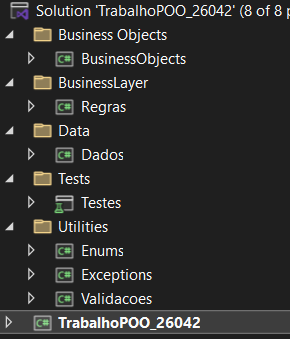
\includegraphics[width=0.5\columnwidth]{N-Tier.png}
	\caption{Design Pattern N-Tier} % Example image
	\end{figure}
	
\subsection{Documentação e comentários}

A \textbf{documentação e os comentários} são componentes fundamentais no desenvolvimento de software, sendo essenciais para a manutenção, compreensão e continuidade de um projeto. Embora o foco principal de um programador seja escrever código funcional e eficiente, garantir que este código seja compreensível para outras pessoas (e até mesmo para o próprio autor no futuro) é igualmente importante. A ausência de uma boa documentação e de comentários claros pode transformar um código funcional em algo difícil de entender e praticamente impossível de manter.

A documentação é importante porque:

\begin{itemize}
	\item \textbf{Facilita a compreensão do Sistema}: Documentar o código e o projeto permite que outros desenvolvedores, sejam eles novos membros da equipa ou colaboradores externos, compreendam rapidamente a estrutura, as funcionalidades e os objetivos do sistema. Sem documentação, entender o propósito e o funcionamento de um código pode exigir um tempo desnecessariamente longo, especialmente em projetos complexos.
	\item \textbf{Reduz Custos de Manutenção}: A maior parte do ciclo de vida de um software envolve a sua manutenção, e um código bem documentado reduz significativamente o tempo necessário para localizar e corrigir problemas, adicionar novas funcionalidades ou fazer atualizações. 
	\item \textbf{Promove a Continuidade do Projeto}: Em situações em que o autor original do código deixa a equipa, a documentação permite que outros programadores continuem o trabalho sem dificuldades. Ela age como um guia que esclarece decisões tomadas, padrões utilizados e os motivos por trás de certas implementações.
	\item \textbf{Evita Ambiguidade}: Mesmo um código bem escrito pode conter complexidades que não são imediatamente óbvias. A documentação serve para esclarecer essas partes, explicando, por exemplo, como um algoritmo específico funciona ou por que uma abordagem foi escolhida em detrimento de outra.
\end{itemize}

\begin{lstlisting}[language={[Sharp]C}, caption={Exemplo de Documentação}, label={Documentação}]
	/// <summary>
	/// Funcao que cria um membro do INEM completo
	/// </summary>
	/// <param name="nomeMembro">Nome do membro</param>
	/// <param name="contacto">Contacto do membro</param>
	/// <param name="email">Email do membro</param>
	/// <param name="especialidade">Especialidade do membro</param>
	/// <returns>Se criou o membro completo com sucesso ou nao</returns>
	public bool CriaMembroINEMCompleto(string nomeMembro, string contacto, string email, EspecialidadeINEM especialidade)
	\end{lstlisting}

\subsection{Utilização do LINQ}

O \textbf{LINQ} (Language Integrated Query) é um conjunto de extensões para as linguagens .NET que introduz uma sintaxe de consulta semelhante ao SQL diretamente no código. Ele permite realizar operações sobre coleções de objetos (como listas, arrays, e dicionários), bases de dados, XML, e até mesmo fontes externas de dados. Isso elimina a necessidade de trabalhar com APIs diferentes para cada tipo de dado, unificando a experiência de desenvolvimento.

As principais caracteristicas são:
\begin{itemize}
	\item \textbf{Sintaxe Uniforme}: 	LINQ oferece uma sintaxe comum para consultar diferentes tipos de dados, como objetos, bases de dados relacionais e documentos XML.
	\item \textbf{Fortemente tipado}:As consultas LINQ são verificadas em tempo de compilação, reduzindo erros e proporcionando maior segurança no código.
	\item \textbf{Composição de consultas}: As consultas podem ser criadas dinamicamente, permitindo compor e reutilizar partes de forma eficiente.
	\item \textbf{Legibilidade}: A sintaxe intuitiva do LINQ torna o código mais fácil de ler e entender, promovendo boas práticas de programação.
\end{itemize}

Com isto o \textbf{LINQ} oferece bastantes benefícios ao nosso código tais como:
\begin{itemize}
	\item \textbf{Redução de Código Boilerplate}: Operações que tradicionalmente exigiriam loops e condições explícitas podem ser realizadas com poucas linhas de código.
	\item \textbf{Integração com o .NET}: LINQ está totalmente integrado ao .NET Framework, utilizando recursos como tipagem forte, IntelliSense e verificações em tempo de compilação.
	\item \textbf{Fácil manutenção}: A legibilidade do código LINQ facilita futuras alterações ou depuração.
	\item \textbf{Uniformidade}: Permite aplicar o mesmo padrão de consultas a diferentes fontes de dados.
\end{itemize}

No desenvolvimento de um projeto, o LINQ facilita significativamente a manipulação de dados, tornando as consultas mais rápidas de escrever e fáceis de entender. Ele é especialmente útil quando se trabalha com grandes coleções de dados ou quando se deseja unificar a lógica de manipulação entre diferentes fontes. Além disso, promove um código mais limpo e alinhado com as boas práticas de programação, sendo uma ferramenta indispensável em projetos que visam eficiência e organização.

\begin{lstlisting}[language={[Sharp]C}, caption={Exemplo de utilização do LINQ}, label={Utilização do LINQ}]
        /// <summary>
/// Funcao que transforma os equipamentos em texto
/// </summary>
/// <returns>Texto que se pretende apresentar</returns>
public override string ToString()
{
	if (equipamentos.Count == 0)
	{
		return "Nao tem equipamentos nesta lista";
	}
	string infoEquip = string.Join("\n", equipamentos.Select(equip => equip.ToString()));
	return infoEquip;
}
\end{lstlisting}

\subsection{Testes}

Os \textbf{testes} desempenham um papel fundamental no desenvolvimento de software, garantindo a qualidade, confiabilidade e manutenção do código. Eles são essenciais para identificar e corrigir erros, validar funcionalidades e assegurar que o sistema atenda aos requisitos especificados. Além disso, ajudam a evitar regressões e a promover boas práticas de programação.

\begin{itemize}
	\item \textbf{Garantia de Qualidade}: Os testes são o principal mecanismo para assegurar que o software funcione conforme esperado. Eles permitem que os desenvolvedores validem se as funcionalidades implementadas cumprem os requisitos e detectem problemas antes que o sistema seja entregue ao cliente ou implantado em produção.
	\item \textbf{Prevenção de regressões}: Conforme o software evolui, com a adição de novas funcionalidades ou correções de bugs, há sempre o risco de introduzir erros em partes já desenvolvidas. Os testes, especialmente os automatizados, ajudam a identificar essas regressões, permitindo que os desenvolvedores façam alterações com maior confiança.
	\item \textbf{Redução de Custos a Longo Prazo}: Embora implementar testes possa parecer um esforço adicional, eles economizam tempo e recursos no longo prazo. Identificar e corrigir um erro durante o desenvolvimento é significativamente menos custoso do que fazer isso após o software ser implementado, onde os custos de manutenção e o impacto nos usuários são muito maiores.
	\item \textbf{Facilidade da Manutenção}: Sistemas bem testados são mais fáceis de manter. Os testes atuam como uma documentação funcional do sistema, fornecendo exemplos claros de como o código deve se comportar em diferentes cenários. Isso é particularmente útil em projetos de longo prazo ou em equipas com alta rotatividade, onde novos desenvolvedores precisam entender rapidamente o funcionamento do sistema.
	\item \textbf{Benefícios na Experiência do Utilizador}:Erros em software podem impactar negativamente a experiência do utilizador, causando insatisfação, perda de confiança e até prejuízos financeiros. Os testes ajudam a evitar problemas críticos, garantindo que o sistema seja estável e ofereça uma experiência fluida e confiável.
\end{itemize}


Os testes não são apenas uma etapa do desenvolvimento, mas uma prática essencial para garantir a qualidade e sustentabilidade de qualquer projeto de software. Eles promovem confiança, reduzem custos e riscos, e permitem que as equipes entreguem soluções robustas e alinhadas às expectativas dos clientes. Investir em testes desde o início do desenvolvimento não é apenas uma boa prática, mas uma abordagem indispensável para o sucesso a longo prazo.

\begin{lstlisting}[language={[Sharp]C}, caption={Exemplo da utilização de testes}, label={Utilização de testes}]
namespace Testes
{
	/// <summary>
	/// Class que contem os testes
	/// </summary>
	[TestClass]
	public sealed class Testes
	{
		/// <summary>
		/// Teste ao construtor da classe Bombeiro
		/// </summary>
		[TestMethod]
		public void Constructor_ParametrosValidos_Bombeiro()
		{
			///Arrange
			string nome = "Joao";
			string contacto = "912345678";
			string email = "joni@gmail.com";
			PatenteBombeiro patente = PatenteBombeiro.OFICIAL;
			
			///Act
			Bombeiro bombeiro = new Bombeiro(nome, contacto, email, patente);
			
			
			///Assert
			Assert.AreEqual(nome, bombeiro.Nome);
			Assert.AreEqual(contacto, bombeiro.Contacto);
			Assert.AreEqual(email, bombeiro.Email);
			Assert.AreEqual(patente, bombeiro.Patente);
			Assert.AreNotEqual(0, bombeiro.Id);
		}
		
		[TestMethod]
		public void Constructor_ParametrosInvalidos_EsperaExcecaoContactoInvalido()
		{
			///Arrange
			string nome = "Joao";
			string contacto = "9123456758";
			string email = "joni@gmail.com";
			PatenteBombeiro patente = PatenteBombeiro.OFICIAL;
			
			///Act & Assert
			try
			{
				Bombeiro bombeiro = new Bombeiro(nome, contacto, email, patente);
				Assert.Fail("Exception esperada nao foi lancada");
			}
			catch (ValidationException e)
			{
				Assert.AreEqual(Erro.CONTACTO_INVALIDO, e.erro);
			}
		}
	}
}

\end{lstlisting}

	\begin{figure}[h] % [h] forces the figure to be output where it is defined in the code (it suppresses floating)
	\centering
	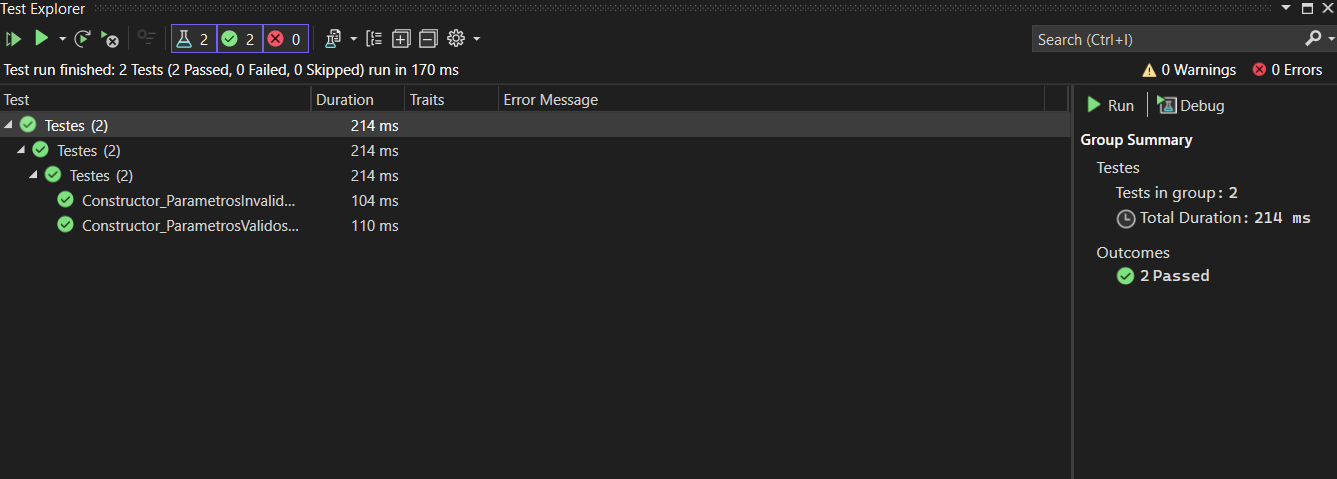
\includegraphics[width=1\columnwidth]{Testes.png}
	\caption{Execução dos testes} % Example image
	\end{figure}
\section{Trabalho desenvolvido}

\subsection{Diagrama de Classes}

\begin{figure}[h] % [h] forces the figure to be output where it is defined in the code (it suppresses floating)
	\centering
	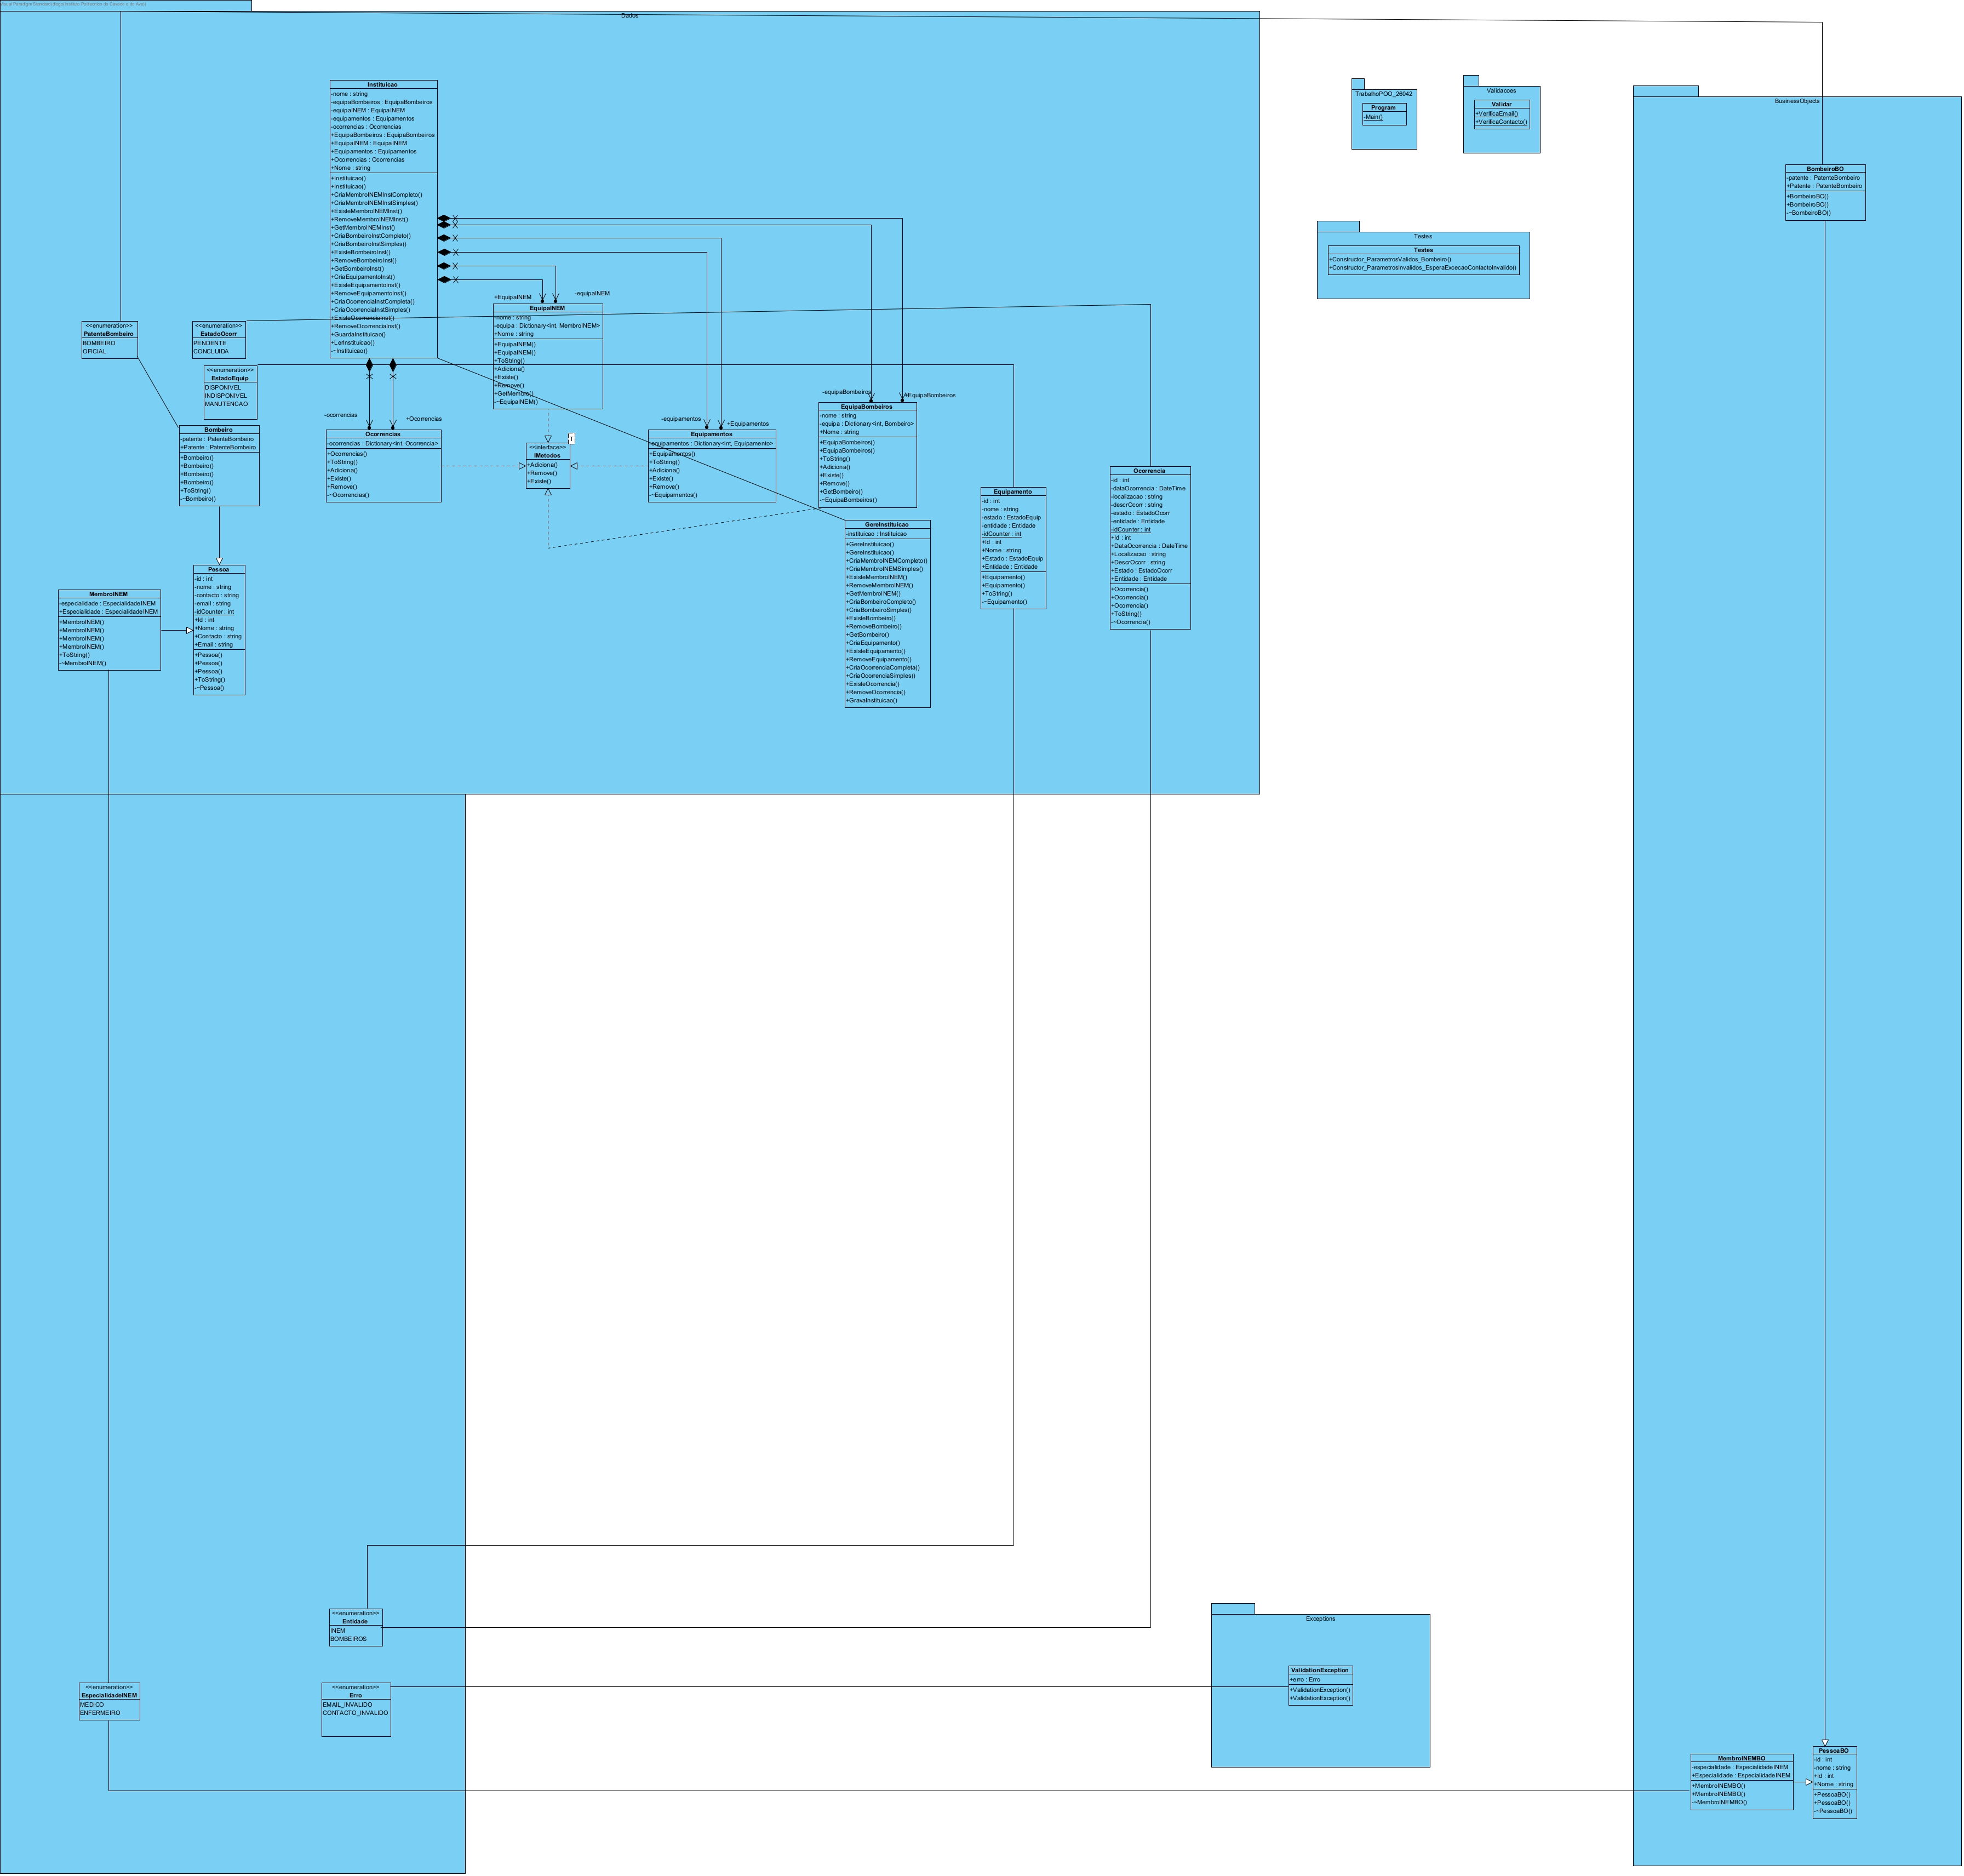
\includegraphics[width=1\columnwidth]{DiagramaUML_POO.png}
	\caption{Diagrama de Classes} % Example image
\end{figure}	

Neste diagrama de classes conseguimos perceber como está estruturado o trabalho desenvolvido. Conseguimos concluir que o programa contém uma camada de dados com todas as estruturas que representam os dados da instituição de proteção civil. De seguida temos a camada de regras que é a camada que o utilizador necessita acessar para conseguir manipular os dados, e consegue isso através da \textit{main} do programa. Com isso ainda contemos ficheiros com funcoes de validacões de alguns dados, como \textit{email} e contacto, ficheiro com enumerados, com alguns enumerados como patente do bombeiro, especialidade do membro do INEM e código de erros, e também um ficheiro com as \textit{exceptions} que serão lançadas no caso de alguns dados estarem inválidos na criação de um objeto. Por fim contém o ficheiro com alguns testes do programa.

\subsection{Estrutura da Solução}

\subsubsection{Bibliotecas (DLL)}

\begin{itemize}
	\item \textbf{Dados.dll}
	\begin{itemize}
		\item \emph{\textbf{Pessoa.cs}}: Definição de atributos e propriedades de pessoa.
		\item \emph{\textbf{Bombeiro.cs}}: Definição de atributos e propriedades de bombeiro. Herda de pessoa.
		\item \emph{\textbf{Bombeiros.cs}}: Classe de agregação de \emph{\textbf{Bombeiro.cs}}, que contém os métodos para gestão do dicionário.
		\item \emph{\textbf{MembroINEM.cs}}: Definição de atributos e propriedades de Membro do INEM. Herda de pessoa.
		\item \emph{\textbf{EquipaINEM.cs}}: Classe de agregação de \emph{\textbf{MembroINEM.cs}}, que contém os métodos para gestão do dicionário.
		\item \emph{\textbf{Equipamento.cs}}: Definição de atributos e propriedades de equipamento.
		\item \emph{\textbf{Equipamentos.cs}}: Classe de agregação de \emph{\textbf{Equipamento.cs}}, que contém os métodos para a gestão do dicionário.
		\item \emph{\textbf{Ocorrência.cs}}: Definição de atributos e propriedades de ocorrência.
		\item \emph{\textbf{Ocorrências.cs}}: Classe de agregação de \emph{\textbf{Ocorrência.cs}}, que contém os métodos para gestão do dicionário.
		\item \emph{\textbf{IMetodos.cs}}: Interface com os métodos utilizados para manipular os dicionários.
		\item \emph{\textbf{Instituicao.cs}}: Classe de agregação com os dicionários com todos os objetos que dizem respeito a uma instituição.
	\end{itemize}
\end{itemize}

\subsubsection{Utilities}

\begin{itemize}
	\item \textit{Validacoes.dll}
	\begin{itemize}
		\item \emph{\textbf{Validacoes.cs}}: Definição dos métodos que dizem respeito à validação de dados que serão inseridos na classe pessoa, nomeadamente o email e contacto.
	\end{itemize}
	\item \textit{Exceptions.dll}
	\begin{itemize}
		\item \emph{\textbf{ValidationException.cs}}: Definição das exceções que serão lançadas no caso dos dados que se validam em \emph{\textbf{Validacoes.cs}} serem inválidos.
	\end{itemize}
	\item \textit{Enums.dll}
	\begin{itemize}
		\item \emph{\textbf{Enumerados.cs}}: Definição dos enumerados que serão utilizados para alguns atributos das classes do \emph{\textbf{Dados.dll}} e para controlo de erros no \emph{\textbf{Exceptions.dll}}.
	\end{itemize}
\end{itemize}

\subsubsection{Business Objects}

\begin{itemize}
	\item \textit{BusinessObjects.dll}
	\begin{itemize}
		\item \emph{\textbf{PessoaBO.cs}}: Definição de atributos de uma pessoa e propriedades que dizem respeito às regras de negócio.
		\item \emph{\textbf{BombeiroBO.cs}}: Definição de atributos de um bombeiro e propriedades que dizem respeito às regras de negócio. Herda de PessoaBO.
		\item \emph{\textbf{MembroINEMBO.cs}}: Definição de atributos de um membro do INEM e propriedades que dizem respeito às regras de negócio. Herda de PessoaBO.
	\end{itemize}
\end{itemize}

\subsubsection{Business Layer}

\begin{itemize}
	\item \textit{Regras.dll}
	\begin{itemize}
		\item \emph{\textbf{GereInstituicao.cs}}: Definição dos métodos da \textit{Business Layer} de modo que o utilizador consiga obter informações dos \emph{\textbf{Dados.dll}} sem ter acesso direto.
	\end{itemize}
\end{itemize}

\subsection{Exemplos do trabalho desenvolvido}

Para os métodos de manipulação de dicionários dos dados foi criada uma interface com os metodos que seriam necessários:
\begin{lstlisting}[language={[Sharp]C}, caption={Demonstração da Interface criada}, label={Interface criada}]
namespace Dados
{
	/// <summary>
	/// Interface que contem as funcoes que serao utilizadas em todas as classes com listas
	/// </summary>
	/// <typeparam name="T">O tipo de objetos que os metodos irao operar</typeparam>
	internal interface IMetodos<T>
	{
		#region Methods
		/// <summary>
		/// Cabecalho da funcao que adiciona um objeto numa lista
		/// </summary>
		/// <param name="item">Objeto que se pretende adicionar</param>
		/// <returns>Se adicionou com sucesso ou nao</returns>
		bool Adiciona(T item);
		
		/// <summary>
		/// Cabecalho da funcao que remove um determinado objeto de uma lista
		/// </summary>
		/// <param name="id">ID do objeto que se pretende remover</param>
		/// <returns>Se removeu com sucesso ou nao</returns>
		bool Remove(int id);
		
		/// <summary>
		/// Cabecalho da funcao que verifica se um determinado objeto existe na lista
		/// </summary>
		/// <param name="id">ID do obejto que se pretende verificar se existe</param>
		/// <returns>Se existe ou nao</returns>
		bool Existe(int id);
		#endregion
	}
}
\end{lstlisting}

Após isso foram implementados os respetivos métodos nas classes de agregação, tal como se pode observar neste exemplo:


\begin{lstlisting}[language={[Sharp]C}, caption={Implementação dos métodos da interface}, label={Métodos da interface}]
namespace Dados 
{
	[Serializable]
	/// <summary>
	/// Purpose: Class EquipaBombeiros que contem um dicionario de bombeiros e o nome da 	equipa
	/// Created by: diogo
	/// Created on: 11/13/2024 7:52:17 PM
	/// </summary>
	/// <remarks></remarks>
	/// <example></example>
	public class EquipaBombeiros : IMetodos<Bombeiro>
	{

			
		/// <summary>
		/// Funcao que adiciona bombeiro no dicionario da equipa de bombeiros
		/// </summary>
		/// <param name="bombeiro">Bombeiro que se pretende adicionar</param>
		/// <returns>Se adicionou com sucesso ou nao</returns>
		public bool Adiciona(Bombeiro bombeiro)
		{
			if(bombeiro == null || Existe(bombeiro.Id))
			{
				return false;
			}
			equipa.Add(bombeiro.Id, bombeiro);
			return true;
		}
			
		/// <summary>
		/// Funcao que verifica se existe um determinado bombeiro na equipa de bombeiros
		/// </summary>
		/// <param name="id">ID do bombeiro que se pretende verificar se existe</param>
		/// <returns>Se existe ou nao</returns>
		public bool Existe(int id)
		{
			return equipa.ContainsKey(id);
		}
		
		
		/// <summary>
		/// Funcao que remove um determinado bombeiro da equipa de bombeiros
		/// </summary>
		/// <param name="id">ID do bombeiro que se pretende remover da equipa</param>
		/// <returns>Se removeu com sucesso ou nao</returns>
		public bool Remove(int id)
		{
			if(Existe(id))
			{
				equipa.Remove(id);
				return true;
			}
			return false;
		}
	}
}
\end{lstlisting}

Para além disso, no caso dos Bombeiros e membros do INEM foi criada uma função que cria o seu respetivo objeto de negócio, de modo a que possam ser enviadas ao utilizador as informações de que ele necessita:

\begin{lstlisting}[language={[Sharp]C}, caption={Implementação do método de criar objeto de negócio}, label={Método que cria objeto de negócio}]
	namespace Dados 
	{
		[Serializable]
		/// <summary>
		/// Purpose: Class EquipaBombeiros que contem um dicionario de bombeiros e o nome da 	equipa
		/// Created by: diogo
		/// Created on: 11/13/2024 7:52:17 PM
		/// </summary>
		/// <remarks></remarks>
		/// <example></example>
		public class EquipaBombeiros : IMetodos<Bombeiro>
		{
			
			/// <summary>
			/// Funcao que devolve as informacoes de um bombeiro da equipa de bombeiros
			/// </summary>
			/// <param name="idBombeiro">Id do bombeiro</param>
			/// <returns>Informacoes do bombeiro</returns>
			public BombeiroBO GetBombeiro(int idBombeiro)
			{
				equipa.TryGetValue(idBombeiro, out Bombeiro bombeiro);
				BombeiroBO bombeiroBO = new BombeiroBO(bombeiro.Id, bombeiro.Nome, bombeiro.Patente);
				return bombeiroBO;
			}
		}
	}
\end{lstlisting}

\newpage
\section{Conclusão}
Neste relatório, foi desenvolvido um sistema para gestão de atividades de socorro, com o objetivo de consolidar conhecimentos no paradigma de programação orientada a objetos e aplicar boas práticas de desenvolvimento de software. Ao longo do trabalho, foram explorados conceitos fundamentais como a utilização de dicionários, princípios SOLID, \textit{design patterns} e validações com LINQ, bem como a importância da documentação e dos testes para a robustez e manutenção do sistema. A aplicação da arquitetura N-Tier foi essencial para a separação de responsabilidades e facilitou a manutenção e evolução do código. Além disso, os testes implementados foram determinantes para assegurar a confiabilidade do sistema.

Em suma, o projeto cumpriu os objetivos propostos, não só fortalecendo a compreensão teórica dos conceitos abordados, mas também permitindo a sua aplicação prática em um contexto próximo ao real. Este trabalho reforça a relevância das boas práticas na programação e a necessidade de continuar a aprimorar as minhas competências no desenvolvimento de soluções robustas e eficientes.

\end{document}
